\documentclass[float=false, crop=true]{standalone}
\usepackage{import}
\usepackage{tikz}
\usepackage{pgfplots}
\usetikzlibrary{calc}
\usepackage{bm}
\usetikzlibrary{arrows}

\begin{document}





\tikzset{every picture/.style={line width=0.75pt}} %set default line width to 0.75pt        

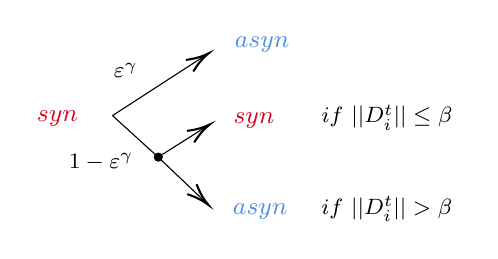
\begin{tikzpicture}[x=0.75pt,y=0.75pt,yscale=-1,xscale=1]
%uncomment if require: \path (0,273); %set diagram left start at 0, and has height of 273

%Straight Lines [id:da8958107357655447] 
\draw    (182.66,91.29) -- (204.66,111.29) ;
%Straight Lines [id:da40222138472283686] 
\draw    (182.66,91.29) -- (227.3,62.38) ;
\draw [shift={(228.98,61.29)}, rotate = 147.07] [color={rgb, 255:red, 0; green, 0; blue, 0 }  ][line width=0.75]    (10.93,-3.29) .. controls (6.95,-1.4) and (3.31,-0.3) .. (0,0) .. controls (3.31,0.3) and (6.95,1.4) .. (10.93,3.29)   ;
%Straight Lines [id:da412726211038148] 
\draw    (204.66,111.29) -- (227.39,132.91) ;
\draw [shift={(228.84,134.29)}, rotate = 223.58] [color={rgb, 255:red, 0; green, 0; blue, 0 }  ][line width=0.75]    (10.93,-3.29) .. controls (6.95,-1.4) and (3.31,-0.3) .. (0,0) .. controls (3.31,0.3) and (6.95,1.4) .. (10.93,3.29)   ;
%Straight Lines [id:da4296406759827529] 
\draw    (204.66,111.29) -- (227.81,96.65) ;
\draw [shift={(229.5,95.58)}, rotate = 147.68] [color={rgb, 255:red, 0; green, 0; blue, 0 }  ][line width=0.75]    (10.93,-3.29) .. controls (6.95,-1.4) and (3.31,-0.3) .. (0,0) .. controls (3.31,0.3) and (6.95,1.4) .. (10.93,3.29)   ;
%Shape: Circle [id:dp3846207107525996] 
\draw  [fill={rgb, 255:red, 0; green, 0; blue, 0 }  ,fill opacity=1 ] (202.81,111.29) .. controls (202.81,110.22) and (203.67,109.36) .. (204.73,109.36) .. controls (205.8,109.36) and (206.66,110.22) .. (206.66,111.29) .. controls (206.66,112.35) and (205.8,113.22) .. (204.73,113.22) .. controls (203.67,113.22) and (202.81,112.35) .. (202.81,111.29) -- cycle ;

% Text Node
\draw (158.14,92.68) node  [font=\small]  {$\textcolor[rgb]{0.82,0.01,0.11}{syn} \ $};
% Text Node
\draw (160.32,108.09) node [anchor=north west][inner sep=0.75pt]  [font=\footnotesize,color={rgb, 255:red, 0; green, 0; blue, 0 }  ,opacity=1 ]  {$1-\varepsilon ^{\gamma }$};
% Text Node
\draw (182,64.62) node [anchor=north west][inner sep=0.75pt]  [font=\footnotesize,color={rgb, 255:red, 0; green, 0; blue, 0 }  ,opacity=1 ]  {$\varepsilon ^{\gamma }$};
% Text Node
\draw (256.78,57.12) node  [font=\small]  {$\textcolor[rgb]{0.29,0.56,0.89}{asyn} \ $};
% Text Node
\draw (255.87,137.46) node  [font=\small]  {$\textcolor[rgb]{0.29,0.56,0.89}{asyn} \ $};
% Text Node
\draw (314.81,136.31) node  [font=\footnotesize,color={rgb, 255:red, 0; green, 0; blue, 0 }  ,opacity=1 ]  {$if\ ||D_{i}^{t} || >\beta $};
% Text Node
\draw (252.87,93.46) node  [font=\small]  {$\textcolor[rgb]{0.82,0.01,0.11}{syn} \ $};
% Text Node
\draw (316.81,92.31) node  [font=\footnotesize,color={rgb, 255:red, 0; green, 0; blue, 0 }  ,opacity=1 ]  {$if\ ||D_{i}^{t} ||\leq \beta \ $};


\end{tikzpicture}


\end{document}